% Default Compiler: txs:///xelatex | txs:///bibtex
% Default Bibliography Tool: BibTex

\documentclass[12pt,onecolumn,a4paper]{article}
\usepackage{listings}
\usepackage{epsfig,graphicx,subfigure,amsthm,amsmath}
\usepackage{caption}
%\usepackage{color}
\usepackage[table, svgnames, usenames,dvipsnames]{xcolor} \usepackage{array}
\usepackage{tabularx}
\usepackage{etoolbox}
\usepackage{cellspace}
\usepackage{float}
\usepackage{hhline}
\usepackage[linktocpage=true,colorlinks,citecolor=blue,pagebackref=true]{hyperref}
\usepackage[top=30mm, bottom=30mm, left=30mm, right=30mm]{geometry}
%\usepackage[T1]{fontenc}
\usepackage[utf8]{inputenc}
\usepackage{fontspec}
\setmainfont{Doulos SIL}
\usepackage{authblk}
\usepackage{polyglossia}
\setotherlanguage{english}
\setotherlanguage{persian}
\usepackage[nonamebreak]{natbib}
\usepackage{xepersian}
\settextfont[Scale=1.2]{IRLotus}
\defpersianfont\mfo[Scale=1.2]{IRLotus}
\setlatintextfont[Scale=1]{Doulos SIL}

\setcounter{Maxaffil}{0}
\renewcommand\Authands{ و }
\renewcommand\Authand{ و }
\renewcommand\Affilfont{\itshape\small}
\providecommand{\keywords}[1]{\textbf{\textit{کلیدواژه‌ها:}} #1}

\setlength\cellspacetoplimit{4pt}
\setlength\cellspacebottomlimit{4pt}
\colorlet{headercolour}{DarkSeaGreen!40}

\DefaultMathsDigits

\definecolor{customblue}{RGB}{235,241,245}
\definecolor{light-gray}{gray}{0.95}
\lstdefinestyle{C++Style}{%
backgroundcolor=\color{customblue},
breaklines=true,
basicstyle=\footnotesize\ttfamily,
keywordstyle=\color{blue},
commentstyle=\color{OliveGreen}\textit,
stringstyle=\color{red},
numbers=left,
numberstyle={\tiny\lr},
showspaces = false,
showstringspaces = false,
tabsize = 2,
frame=single,
xleftmargin=5pt,
xrightmargin=3pt,
language = C++,
aboveskip = 20pt,
rulecolor=\color{black},
captiondirection=RTL,
}

\lstnewenvironment{C++Code}[1][]
{%
\lstset{style=C++Style, #1}%
}{%
}

\def\lstlistingname{شبه‌کد}

\begin{document}
    \title{تشخیص خودکار وزن عروضی اشعار کلاسیک فارسی\footnote{دومین همایش ملی آموزش زبان فارسی و زبان‌شناسی، شیراز، اردیبهشت 1392}}
    \author[1]{وحید مواجی}
    \author[2]{محرم اسلامی}
    \affil[1]{دانشگاه صنعتی شریف}
    \affil[2]{دانشگاه زنجان}
    \date{25 اردیبهشت 1392}
    \maketitle

    \begin{abstract}
        در مقالۀ حاضر می‌کوشیم وزن عروضی اشعار کلاسیک فارسی را به طور خودکار و ماشینی تعیین کنیم. برخورداری خط فارسی از ویژگی‌هایی چون عدم نمایش واکه‌های کوتاه و به دنبال آن موضوع هم‌نویسگی، مسأله کسره اضافه، فاصله بینِ اجزای کلمه واحد، فقدان فاصله بین کلمه‌های مستقل، موضوعِ جدانویسی و پیوسته‌نویسی و غیره موجب می‌شود قبل از انجام هرگونه پردازشی، متون فارسی را به زنجیره واجی تبدیل کنیم. بدین منظور با استفاده از تحلیل‌گر صرفی پارس-مورف که توسط نگارندگان طراحی و پیاده‌سازی شده است، متن ورودی از لحاظ صرفی تحلیل شده و اجزای صرفی آن از قبیل پیشوندها، پسوندها، اشتقاق و ترکیب بدست آمده و سپس با استفاده از واژگان زایای زبان فارسی {\mfo\citep{eslami_83}}، صورت واجی‌ آنها با هم ترکیب شده و در نهایت صورت واجی متن ورودی به‌دست می‌آید. سپس این زنجیره واجی را طبق روش‌های موجود در عروض فارسی تقطیع هجایی و تقطیع به ارکان کرده و در ادامه با استفاده از الگوریتم لونشتاین که الگوریتمی برای یافتن حداقل فاصله بین دو رشته است، در بین گروه‌های وزنی که گردآوری کرده‌ایم، آن گروهی که کمترین فاصله را با تقطیع متن مورد نظر دارد انتخاب کرده و وزن مناسب را مطابق با آن می‌یابیم. از آنجا که خط فارسی فاقد مصوت‌ها است، لذا دقت الگوریتم ممکن است بسته به نمود واجی که پیشنهاد می‌دهد تغییر کند یا کاهش یابد. به همین دلیل این امکان در برنامه فراهم شده است که شعر را به صورت زنجیره واجی نیز وارد نموده و وزن آن را تعیین کنیم. در این کار از 31 وزن رایج و پرکاربرد زبان فارسی استفاده کرده‌ایم. از کاربردهای برنامه تشخیص خودکار وزن عروضی می‌توان به آموزش عروض به فارسی زبانان و غیر فارسی‌زبانان، بررسی صحت و دقت تعیین وزن عروضی اشعار به روش‌های سنتی و ارائه شیوه‌های مختلف خوانش اشعار کلاسیک فارسی اشاره نمود.
        \par
        \keywords{تحلیل‌گر صرفی، زنجیره واجی، تشخیص خودکار، وزن عروضی، الگوریتم لونشتاین، شعر فارسی.}
    \end{abstract}

    \section{مقدمه}
    در این پژوهش سعی بر این داریم تا با استفاده از فناوری رایانه و روش‌های زبان‌شناسی رایانشی، وزن شعر کلاسیک فارسی را تعیین کنیم. از آنجا که در شعر کلاسیک، وزن مصراع معیار است، لذا ورودی این برنامه «مصراع» می‌باشد نه «بیت». یکی از نیازمندی‌های چنین برنامه‌ای داشتن قابلیت تبدیل متن فارسی به زنجیره واجی می‌باشد. روش‌های متعددی برای تبدیل متن به زنجیره واجی مورد استفاده قرار گرفته است. در \Latincite{allen_1992} از قواعد تبدیل نویسه به صورت واجی استفاده شده و استثنائات نیز از یک فرهنگ استخراج می‌شود. استفاده از یک درخت تصمیم چندسطحی که هر نویسه را نسبت به حروف مجاور آن به صورت یک درخت نمایش می‌دهد در \Latincite{torkkola_1993} مورد مطالعه قرار گرفته است. استفاده از روش‌های زبان طبیعی نیز مورد بررسی قرار گرفته است. در این روش، هر تکواژ به همراه اطلاعات مربوط به صورت‌های صرفی مختلف آن مانند صورت جمع، گذشته، حال، و غیره و کلیه اطلاعات صرفی مربوطه در یک دادگان ذخیره می‎‌شود. در این حالت نیز اگر کلمه در فهرست تکواژها نباشد از قواعد تبدیل نویسه به صورت واجی یا فرهنگ استثناها استفاده می‌شود {\mfo\citep{sayad_75}}.
    \par
    یکی از روش‌های تبدیل خودکار متن فارسی به زنجیره واجی، استفاده از یک تحلیل‌گر صرفی است. در این روش با استفاده از یک تحلیل‌گر صرفی، عبارت ورودی به اجزای تشکیل‌دهنده آن تقطیع شده و سپس هر قطعه به عنوان ورودی به تحلیل‌گر صرفی داده می‌شود تا به اجزای صرفی تشکیل‌دهنده‌اش از قبیل پسوندها و پیشوندهای تصریفی و اشتقاقی، پایه‌های ترکیب و اشتقاق و غیره تجزیه شود و سپس صورت واجی اجزا با هم ترکیب شده و زنجیره واجی کل متن به دست می‌آید.
    \par
    در این مقاله از روش تحلیل‌گر صرفی برای تبدیل متن فارسی به زنجیره واجی استفاده شده است. سپس زنجیره واجی تقطیع هجایی و تقطیع به ارکان شده و به صورت رشته‌ای از (-)ها و \rl{(U)}ها درمی‌آید که به ترتیب نمایانگر هجاهای بلند و هجاهای کوتاه هستند. بعد از این مرحله، رشته ورودی با استفاده از الگوریتم لونشتاین با مجموعه‌ای از گروه‌های وزنی پرکاربرد زبان فارسی مقایسه می‌شود و رشته‌ای که کمترین فاصله یا به عبارت دیگر بیشترین مشابهت را با رشته ورودی داشته باشد به عنوان وزن عروضی انتخاب می‌شود. لازم به ذکر است که در نسخه اولیه برنامه، مواردی همچون «اختیارات شاعری»، «اختیارات وزنی»، و «عروض نیمایی» پشتیبانی نمی‌شود.

    \section{تبدیل متن فارسی به زنجیره واجی}
    در این تحقیق از تحلیل‌گر صرفی پارس مورف {\mfo\citep{mavaji_90}} برای تبدیل متن فارسی به زنجیره واجی استفاده شده است. در طراحی پارس مورف، ساخت تصریفی کلمه در زبان فارسی {\mfo\citep{eslami_88}} به صورت ساختمند در نظر گرفته شده است و جایگاه طبقات مختلف وندهای تصریفی در ساختمان انواع کلمات مشخص شده است. پارس مورف در تحلیل تصریفی کلمه ابتدا ستاک را شناسایی می‌کند و متناسب با ساخت تصریفی پیش‌بینی شده برای آن نوع ستاک به دنبال انواع وندهای تصریفی در جایگاه‎‌های خاص، با در نظر گرفتن صورت‌های مختلف نوشتاری هرکدام از طبقات، می‌گردد.
    \par
    اگر ستاک پیچیده باشد، پارس مورف با اعمال قواعد واژه‌سازی زبان فارسی، ستاک مورد نظر را از حیث مشتق یا مرکب بودن تجزیه و تحلیل و اجزای سازنده آن را با ذکر مقوله دستوری و نقش آنها مشخص می‌کند. به دلیل معتبر نبودن فاصله به عنوان مرز کلمه در متون فارسی، پارس مورف در تجزیه ستاک‌های پیچیده، ترکیب‌های بالقوه را نیز به عنوان گزینه‌های بعدی در اختیار می‌گذارد.
    \par
    در برنامه تحلیل‌گر صرفی پارس مورف این امکان وجود دارد که متن فارسی به عنوان ورودی برنامه داده شده و نتیجه به صورت زنجیره واجی نشان داده ‌شود. برای علائم واجی زبان فارسی از علائم موجود در {\mfo\citep{samareh_78}} استفاده کرده‌ایم. مثلاً واج‌های  \lr{ʔ}، \lr{š}، \lr{â}، \lr{ĵ} ، \lr{č} و \lr{ž} به ترتیب نمایانگر نویسه‌های /همزه/، /ش/، /آ/، /ج/، /چ/ و /ژ/ می‌باشند.
    \par
    خروجی این برنامه برای جمله «آن یکی نحوی به کشتی درنشست» در جدول \ref{table:1} آمده است. همانطور که مشاهده می‌گردد، دو صورت واجی برای این عبارت نشان داده شده است که در یکی کلمه «کشتی» به صورت \lr{/ kašti /} و در دیگری به صورت \lr{/ kešti /} واج‌نویسی شده است.

    \begin{table}[H]
        \centering
        \caption{زنجیره واجی عبارت «آن یکی نحوی به کشتی درنشست»}
        \label{table:1}
        \begin{tabular}{| c | r |}
            \hline
            \lr{ʔân yeki nahvi beh kašti dar nešast} \\
            \hline
            \lr{ʔân yeki nahvi beh kešti dar nešast} \\
            \hline
        \end{tabular}
    \end{table}

    \par
    در جدول \ref{table:2}، زنجیره واجی عبارت «مردم حضور دارند» آمده است. در این حالت هم دو نوع واج‌نویسی برای کلمه «مردم» آمده است: اولی دارای مقوله دستوری اسم است که به صورت /mardom/ نوشته شده و دیگری نتیجه تحلیل صرفی به صورت فعل «مردن» در حالت اول شخص مفرد است یعنی mord+am. از آنجا که تحلیل نحوی روی عبارت ورودی انجام نمی‌شود، این زنجیره واجی نیز از لحاظ برنامه معتبر است. ولی با افزودن اطلاعات نحوی به برنامه می‌توان دقت آن را بالاتر برد.

    \begin{table}[H]
        \centering
        \caption{زنجیره واجی عبارت «مردم حضور دارند»}
        \label{table:2}
        \begin{tabular}{| c | r |}
            \hline
            \lr{mardom hozur dârand} \\
            \hline
            \lr{mordam hozur dârand} \\
            \hline
        \end{tabular}
    \end{table}

    \par
    مسأله بعدی، مسأله کسره اضافه است که باید تمهیدی برای آن اندیشیده شود. چون کسره اضافه در متن فارسی نمایش داده نمی‌شود، ولی در زنجیره واجی حضور دارد؛ لازم است اطلاعات نحوی به برنامه تبدیل متن به زنجیره واجی اضافه شود تا دقت برنامه افزایش یابد. برای مثال در جدول \ref{table:3} خروجی برنامه به ازای عبارت «کتاب من کو؟» آورده شده که در آن کسره اضافه را نمی‌بینیم.

    \begin{table}[H]
        \centering
        \caption{زنجیره واجی عبارت «کتاب من کو؟»}
        \label{table:3}
        \begin{tabular}{| c | r |}
            \hline
            \lr{ketâb man ku} \\
            \hline
        \end{tabular}
    \end{table}

    \section{تقطیع}
    هجاهای فارسی از نظر امتداد سه نوعند: هجای کوتاه، هجای بلند، هجای کشیده {\mfo\citep{soltani_90}}. هجای کوتاه دارای دو واج است (صامت + مصوت کوتاه) و با (U) نمایش داده می‌شود. هجای بلند دارای سه واج است (و یا یک صامت + یک مصوت بلند) که با علامت (-) نمایش داده می‌شود. هجای کشیده بیش از سه واج دارد و با علامت \rl{(U-)} نمایش داده می‌شود و از نظر امتداد معادل یک هجای بلند و یک هجای کوتاه است.
    \par
    در تعیین وزن شعر فارسی اگر وزن یک مصراع (در شعر کلاسیک) را به‌دست آوریم، وزن شعر به‌دست آمده است. علت آن است که در زبان فارسی هم مثل بسیاری از زبان‌ها، واحد وزن شعر مصراع است. یعنی وقتی شاعر مصراع اول شعر را سرود وزن شعرش را انتخاب کرده است. در بقیه مصراع‌ها همان وزن باید تکرار شود.

    \subsection{تقطیع هجایی}
    منظور از تقطیع هجایی آن است که مصراع‌های مورد نظر را به هجاهای تشکیل‌دهنده آن تقسیم کنیم. برای این کار ابتدا مصراع‌های مورد نظر را به خط عروضی می‌نویسیم، سپس آن را به هجاهای تشکیل دهنده‌اش تقسیم می‌کنیم.
    مثال در جدول \ref{table:4}:

    \begin{table}[H]
        \caption{مبند ای دل به جز در یار خود دل / امید از هر که داری جمله بگسل}
        \label{table:4}
        \centering\setLTR
        \begin{tabularx}{\textwidth}{|X|X|X|X|X|X|X|X|X|X|X|X|X|X|X|X|X|X|X|X|X|X|}
            \hline
            \rl{سِل} & \rl{بُگ} & \rl{لِ} & \rl{جُم} & \rl{ری} & \rl{دا} & \rl{کِ} & \rl{هَر} & \rl{دَز} & \rl{می} & \rl{اُ} & \rl{دِل} & \rl{خُد} & \rl{رِ} & \rl{یا} & \rl{دَر} & \rl{جُز} & \rl{بِ} & \rl{دِل} & \rl{دی} & \rl{بَن} & \rl{مَ}  \tabularnewline \hline
            - & - & U & - & - & - & U & - & - & - & U & - & - & U & - & - & - & U & - & - & - & U  \tabularnewline \hline
        \end{tabularx}
        \setRTL
    \end{table}

      \subsection{تقطیع به ارکان}
    در تقطیع به ارکان، هجاهای مصراع‌ها را سه‌تا سه‌تا یا چهارتا چهارتا یا سه‌تا چهارتا یا چهارتا سه‌تا تقسیم می‌کنند. تقسیم‌بندی‌های دیگر در عروض امروز رایج نیست. علت آن است که بیشتر کلمات فارسی حداکثر چهار هجا دارند و کلماتی که بیش از چهار هجا دارند بسیار کم‌اند. همچنین تقسیم‌بندی چهارتا سه‌تا بسیار نامتداول است. مثال در جدول \ref{table:5}:

    \begin{table}[H]
        \scriptsize
        \caption{باور مکن که من دست از دامنت بدارم / شمشیر نگسلاند پیوند مهربانان}
        \label{table:5}
        \centering\setLTR
        \begin{tabularx}{\textwidth}{|X|X|X|X|X|X|X|X|X|X|X|X|X|X|X|X|X|X|X|X|X|X|X|X|X|X|X|}
            \hline
            \rl{نان} & \rl{با} & \rl{رَ} & \rl{مِه} & \rl{دِ} & \rl{وَن} & \rl{پی} & \rl{نَد} & \rl{لا} & \rl{سَ} & \rl{نَگ} & \rl{شیر} & \rl{شَم} & \rl{رَم} & \rl{دا} & \rl{بِ} & \rl{نَت} & \rl{مَ} & \rl{دا} & \rl{تَز} & \rl{دَس} & \rl{مَن} & \rl{کِ} & \rl{کُن} & \rl{مَ} & \rl{وَر} & \rl{با}  \tabularnewline \hline
            - & - & U & - & U & - & - & - & - & U & - & {U-} & - & - & - & U & - & U & - & - & - & - & U & - & U & - & -   \tabularnewline \hline
        \end{tabularx}
        \setRTL
    \end{table}

    \par
    حال می‌توان به جای هجاهای کوتاه و بلند از (-) و (U) استفاده کنیم. البته چون در صرف و نحو عربی همه کلمات را با «ف، ع، ل» می‌سنجند، در عروض عربی و فارسی هم وزن هجاهای تقطیع شده هر مصراع را (که نمایانگر نظم وزن‌اند) از «ف، ع، ل» ساخته‌اند {\mfo\citep{soltani_90}}. مثلاً هم‌وزن (--U) فَعولن است. همچنین به جای (---U) از قالب هم‌وزنش «مفاعیلن» استفاده می‌کنند. مهمترین قالب‌ها یا ارکان عروضی را وحیدیان کامکار نوزده تا دانسته است {\mfo\citep{vahidian_65}}.

    \section{فاصلۀ لونشتاین\protect\LTRfootnote{\lr{Levenshtein distance}}}\label{sec:4}
    فاصلۀ لونشتاین \Latincite{levenshtein_1966} به صورت حداقل میزان تغییرات مورد نیاز برای رشتۀ S به رشتۀ T تعریف می‌شود که عملیات مجاز در آن عبارتند از: درج، حذف یا جانشینی یک نویسۀ واحد. برای مثال فاصلۀ لونشتاین دو رشتۀ \lr{apple} و \lr{orange} با یک ماتریس ساده در جدول \ref{table:6} محاسبه شده است. فاصلۀ این دو رشته برابر 5 است که در قسمت پایین و سمت راست ماتریس نشان داده شده است. این فاصله بدین معناست که رشتۀ \lr{apple} را با درج \lr{o}، جانشینی \lr{r} به جای \lr{a}، \lr{a} به جای \lr{p}، \lr{n} به جای \lr{p} و \lr{g} به جای \lr{l} به رشتۀ \lr{orange} تبدیل می‌شود. یک عملیات درج و چهار عملیات جانشینی داریم که مجموعاً برابر 5 می‌شود.


    \begin{table}[H]
        \caption{مثالی از فاصلۀ لونشتاین}
        \label{table:6}
        \centering\setLTR
        \begin{tabular}{c|ccccccc|}
            \multicolumn{1}{c}{} & \multicolumn{1}{c}{} & \cellcolor{blue!25}A & \cellcolor{blue!25}P & \cellcolor{blue!25}P & \cellcolor{blue!25}L & \cellcolor{blue!25}E \tabularnewline \hhline{~|*{6}{-}}
            & 0 & 1 & 2 & 3 & 4 & 5  \tabularnewline
            \cellcolor{blue!25}O & 1 & 1 & 2 & 3 & 4 & 5   \tabularnewline
            \cellcolor{blue!25}R & 2 & 2 & 2 & 3 & 4 & 5   \tabularnewline
            \cellcolor{blue!25}A & 3 & 2 & 3 & 3 & 4 & 5   \tabularnewline
            \cellcolor{blue!25}N & 4 & 3 & 3 & 4 & 4 & 5   \tabularnewline
            \cellcolor{blue!25}G & 5 & 4 & 4 & 4 & 5 & 5   \tabularnewline
            \cellcolor{blue!25}E & 6 & 5 & 5 & 5 & 5 & 5   \tabularnewline
        \end{tabular}
        \setRTL
    \end{table}

    \par
    مراحل ساخته شدن ماتریس شکل 1 به شرح ذیل است:
    \begin{enumerate}
        \item ماتریس $d$ با $M$ سطر و $N$ ستون ساخته می‌شود.
        \item به سطر اول مقادیر از $0$ تا $M$ و به ستون اول مقادیر از $0$ تا $N$ اختصاص داده می‌شود.
        \item هر نویسه‌ای از $S$ ($i$ از $1$ تا $M$)  و هر نویسه‌ای از $T$ ($j$ از $1$ تا $N$) را بررسی می‌کنیم.
        \item اگر $S[i]$ با $T[j]$ برابر بود، هزینه برابر $0$ و در غیر این صورت برابر $1$ است.
        \item مقدار عنصر $d[i, j]$ ماتریس برابر کمینه مقادیر زیر است:
        \begin{enumerate}
            \item عنصر بالایی بعلاوۀ یک: $d[i-1, j]+1$
            \item عنصر سمت چپ بعلاوۀ یک: $d[i, j-1]+1$
            \item عنصر بالا و سمت چپ بعلاوۀ هزینه: $d[i-1, j-1]+cost$
        \end{enumerate}
        \item بعد از این که تکرار مراحل 3، 4 و 5 به پایان رسید، مقدار فاصله در عنصر $d[N,M]$ قرار دارد.
    \end{enumerate}

    \par
    شبه‌کد فاصلۀ لونشتاین در شبه‌کد \ref{listing:1} آمده است.

    \begin{LTR}
        %@formatter:off
        \begin{lstlisting}[style=C++Style,caption=\rl{فاصلۀ لونشتاین}, label={listing:1}]
        int LevenshteinDistance(char S[1..M], char T[1..N]){
            declare int d[0..M, 0..N]
            for i from 0 to M
                d[i,0] := i //the distance of any first string to an empty second string
            for j from 0 to N
                d[0, j] := j //the distance of any second string to an empty first string
            for j from 1 to N
            {
                for i from 1 to M
                {
                    if S[i] = T[j] then
                        d[i, j] := d[i-1, j-1] //no operation required
                    else d[i, j] := minimum(d[i-1, j] + 1, //a deletion
                                d[i, j-1] + 1, //an insertion
                                d[i-1, j-1] + 1) //a substitution
                }
            }
            return d[M, N]
        }
        \end{lstlisting}
        %@formatter:on
    \end{LTR}

    \section{پیاد‌ه‌سازی}
    با توجه به مبانی نظری که به طور خلاصه در بخش‌های قبل ذکر شد، برنامه‌ای طراحی گردید که متن ورودی را گرفته و مراحل تقطیع هجایی و تقطیع به ارکان آن را انجام می‌دهد. البته اگر متن ورودی به خط فارسی باشد، ابتدا به زنجیرۀ واجی تبدیل می‌شود. با توجه به الگوی واجی زبان فارسی که به صورت‌های \lr{CV}, \lr{CVC}, \lr{CVCC} است، هر گاه مصوتی پیدا شود، صامت قبل از آن متعلق به آن بوده و چون خوشه‌های همخوانی در آغازه هجا نداریم، لذا صامت‌های قبل از آن متعلق به هجای قبلی خواهند بود. بدین ترتیب مصراع ورودی به صورت رشته‌ای از (-)ها و \rl{(U)}ها تبدیل می‌شود. سپس با استفاده از الگوریتم لونشتاین که در بخش \ref{sec:4} شرح داده شد، در بین گروه‌های وزنی که در جدول \ref{table:7} آمده‌اند، آن گروهی که کمترین فاصله را با متنِ تقطیع شده دارد انتخاب کرده و به عنوان وزن شعر (مصراع) برمی‌گردانیم. در حقیقت، اگر هر کدام از گروه‌های وزنی را به صورت رشته‌ای از (-) و \rl{(U)}ها در نظر بگیریم، آنگاه مسأله پیدا کردن وزن عروضی به مسأله پیدا کردن رشته‌ای با کمترین فاصله یا بیشترین مشابهت با رشته ورودی کاهش می‌یابد.
    \par
    در شکل \ref{fig:1} نمونه‌ای از خروجی برنامه را هم به صورت ورودی خط فارسی و هم ورودی واج‌نویسی شده برای رشته ورودی «آن یکی نحوی به کشتی درنشست» می‌بینیم که وزن «فاعلاتن فاعلاتن فاعلن» را به عنوان خروجی ارائه داده است. همانگونه که در شکل \ref{fig:1} می‌بینیم، ابتدا متن ورودی به زنجیره واجی تبدیل شده، و بعد از اعمال تقطیع به صورت رشته‌ای از (-) و \rl{(U)}ها درآمده است و نهایتاً با استفاده از الگوریتم لونشتاین، گروه وزنی آن مشخص شده است. به دلیل عدم نوشتن مصوت‌ها در خط فارسی و به تبع آن وجود نمودهای واجی مختلف برای یک رشته واحد ممکن است دقت الگوریتم بسته به نمود واجی که پیشنهاد می‌دهد تغییر کند یا کاهش یابد. به همین دلیل این امکان در برنامه فراهم شده است که شعر را به صورت زنجیره واجی نیز وارد نموده و وزن آن را تعیین کنیم.

    \begin{figure}[H]
        \centering
        \makebox[\textwidth]{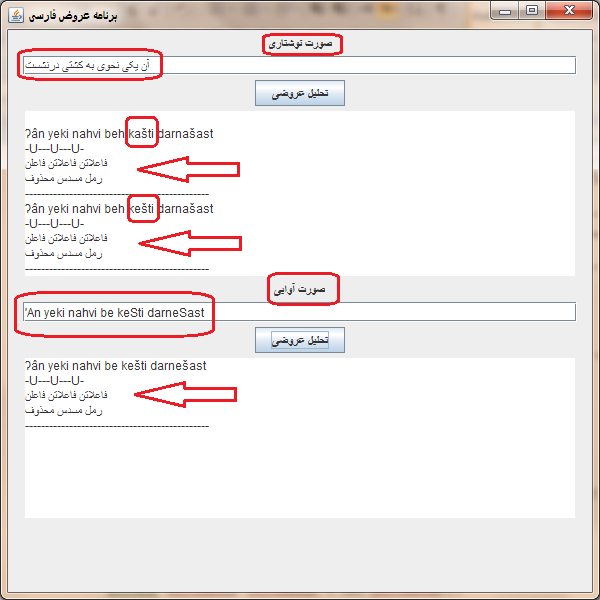
\includegraphics[width=\textwidth]{fltl1.png}}
        \caption{خروجی نمونه برنامه برای مصراع «آن یکی نحوی به کشتی درنشست»}
        \label{fig:1}
    \end{figure}

    \begin{table}[H]
        \caption{وزن‌های پرکاربرد در زبان فارسی}
        \label{table:7}
        \centering\setLTR
        \begin{tabular}{|c|c|c|}
            \hline
            \cellcolor{blue!25}\rl{نام گروه وزنی} & \cellcolor{blue!25}\rl{گروه وزنی} & \cellcolor{blue!25}\rl{تقطیع} \tabularnewline \hline
            \rl{رمل مثمن مخبون محذوف} & \rl{فعلاتن فعلاتن فعلاتن فعلن} & \lr{UU--UU--UU--UU-} \tabularnewline \hline
            \rl{مجتث مثمن محذوف} & \rl{مفاعلن فعلاتن مفاعلن فعلن} & \rl{U-U-UU--U-U-UU-} \tabularnewline \hline
            \rl{مضارع مثمن اخرب مكفوف محذوف} & \rl{مفعول فاعلات مفاعیل فاعلن} & \rl{--U-U-UU--U-U-} \tabularnewline \hline
            \rl{رمل مثمن محذوف} & \rl{فاعلاتن فاعلاتن فاعلاتن فاعلن} & \rl{-U---U---U---U-} \tabularnewline \hline
            \rl{هزج مثمن سالم} & \rl{مفاعیلن مفاعیلن مفاعیلن مفاعیل} & \rl{U---U---U---U--U} \tabularnewline \hline
            \rl{هزج مسدس محذوف} & \rl{مفاعیلن مفاعیلن فعولن} & \rl{U---U---U--} \tabularnewline \hline
            \rl{مضارع مثمن اخرب} & \rl{مفعول فاعلاتن مفعول فاعلاتن} & \rl{--U-U----U-U--} \tabularnewline \hline
            \rl{هزج مثمن اخرب مكفوف محذوف} & \rl{مفعول مفاعیل مفاعیل فعولن} & \rl{--UU--UU--UU--} \tabularnewline \hline
            \rl{خفیف مخبون محذوف} & \rl{فعلاتن مفاعلن فعلن} & \rl{UU--U-U-UU-} \tabularnewline \hline
            \rl{رمل مسدس محذوف} & \rl{فاعلاتن فاعلاتن فاعلن} & \rl{-U---U---U-} \tabularnewline \hline
            \rl{رجز مثمن مطوی مخبون} & \rl{مفتعلن مفاعلن مفتعلن مفاعلن} & \rl{-UU-U-U--UU-U-U-} \tabularnewline \hline
            \rl{هزج مثمن اخرب} & \rl{مفعول مفاعیلن مفعول مفاعیلن} & \rl{--UU-----UU---} \tabularnewline \hline
            \rl{رمل مثمن مشكول} & \rl{فعلات فاعلاتن فعلات فاعلاتن} & \rl{UU-U-U--UU-U-U--} \tabularnewline \hline
            \rl{مجتث مثمن مخبون} & \rl{مفاعلن فعلاتن مفاعلن فعلاتن} & \rl{U-U-UU--U-U-UU--} \tabularnewline \hline
            \rl{هزج مسدس اخرب مقبوض محذوف} & \rl{مفعول مفاعلن فعولن} & \rl{-UU-U-U-} \tabularnewline \hline
            \rl{متقارب مثمن اثلم} & \rl{مستفعلاتن مستفعلاتن} & \rl{--U----U--} \tabularnewline \hline
            \rl{منسرح مثمن مطوی منحور} & \rl{مفتعلن فاعلات مفتعلن فع} & \rl{-UU--U-U-UU--} \tabularnewline \hline
            \rl{رجز مثمن سالم} & \rl{مستفعلن مستفعلن مستفعلن مستفعلن} & \rl{--U---U---U---U-} \tabularnewline \hline
            \rl{منسرح مثمن مطوی مكشوف} & \rl{مفتعلن فاعلن مفتعلن فاعلن} & \rl{-UU--U--UU--U-} \tabularnewline \hline
            \rl{مقتضب مثمن مطوی مقطوع} & \rl{فاعلات مفعولن فاعلات مفعولن} & \rl{-U-U----U-U---} \tabularnewline \hline
            \rl{سریع مطوی مكشوف} & \rl{مفتعلن مفتعلن فاعلن} & \rl{-UU--UU--U-} \tabularnewline \hline
            \rl{متقارب مثمن سالم} & \rl{فعولن فعولن فعولن فعولن} & \rl{U--U--U--U--} \tabularnewline \hline
            \rl{متقارب مثمن محذوف} & \rl{فعولن فعولن فعولن فعل} & \rl{U--U--U--U-} \tabularnewline \hline
            \rl{رجز مثمن مطوی} & \rl{مفتعلن مفتعلن مفتعلن مفتعلن} & \rl{-UU--UU--UU--UU-} \tabularnewline \hline
            \rl{رمل مثمن مخبون} & \rl{فعلاتن فعلاتن فعلاتن فعلاتن} & \rl{UU--UU--UU--UU--} \tabularnewline \hline
            \rl{رمل مسدس مخبون محذوف} & \rl{فعلاتن فعلاتن فعلن} & \rl{UU--UU--UU-} \tabularnewline \hline
            \rl{هزج مثمن مكفوف محذوف} & \rl{مفاعیل مفاعیل مفاعیل فعولن} & \rl{U--UU--UU--UU--} \tabularnewline \hline
            \rl{خفیف مثمن مخبون} & \rl{فعلاتن مفاعلن فعلاتن مفاعلن} & \rl{UU--U-U-UU--U-U-} \tabularnewline \hline
            \rl{هزج مسدس اخرب مقبوض} & \rl{مفعول مفاعلن مفاعیلن} & \rl{--UU-U-U---} \tabularnewline \hline
            \rl{رمل مثمن سالم} & \rl{فاعلاتن فاعلاتن فاعلاتن فاعلاتن} & \rl{-U---U---U---U--} \tabularnewline \hline
            \rl{بسیط مثمن مخبون} & \rl{مستفعلن فعلن مستفعلن فعلن} & \rl{--U-UU---U-UU-} \tabularnewline \hline
        \end{tabular}
        \setRTL
    \end{table}

    \section{نتیجه‌گیری}
    در این مقاله، با استفاده از سامانه تحلیل‌گر صرفی کلمه در زبان فارسی با عنوان پارس مورف، که بر پایه یک مطالعه دقیق زبان‌شناختی از نظام صرفی زبان فارسی استوار است، سعی کردیم تا فرایند خودکار تبدیل متن فارسی به زنجیره واجی را توسعه دهیم و با استفاده از آن عمل تقطیع هجایی و تقطیع به ارکان را روی متن ورودی انجام دهیم. سپس با درنظر گرفتن تقطیع متن ورودی و گروه‌های وزنی پرکاربرد به صورت رشته‌ای از (-) و \rl{(U)}ها و کاهش مسأله به مسألۀ یافتن کمترین فاصله بین دو رشته و بکارگیری الگوریتم لونشتاین، وزن عروضی مصراع ورودی را به دست آوردیم.
    \par
    از چالش‌های پیش رو که در کارهای آتی باید به آنها پرداخته شود، درنظر گرفتن دشواری‌های موجود در پردازش متن فارسی {\mfo\citep{eslami_81}} است که باید راهکارهایی برای حل آن اندیشیده شود تا دقت الگوریتم تبدیل متن فارسی به زنجیرۀ واجی و به تبع آن دقت مراحل تقطیع و یافتن وزن عروضی افرایش یابد. در کارهای آتی می‌توان مواردی همچون «اختیارات شاعری»، «اختیارات وزنی»، و «عروض نیمایی» را به امکانات برنامه افزود. از نتایج این تحقیق می‌توان به عنوان یک برنامه کمک آموزشی در زمینه‌های آموزش عروض به فارسی زبانان و غیر فارسی‌زبانان، بررسی صحت و دقت تعیین وزن عروضی اشعار به روش‌های سنتی و ارائه نحوه‌های مختلف خوانش اشعار کلاسیک فارسی اشاره نمود.
    {\mfo
    \bibliographystyle{asa-fa}
    \bibliography{references}}

\end{document}